\documentclass{standalone}

\usepackage{tikz}
\usepackage{tkz-euclide}

\usepackage{times}

\begin{document}
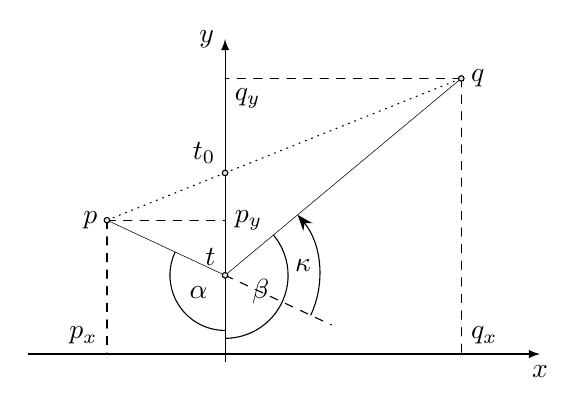
\begin{tikzpicture}[%
  line/.style = {thin, dashed},
  >={Stealth[scale=1.2]},
]
  \tkzInit[xmin=-2.5,xmax=3.5,ymin=-0.1,ymax=3.5]
  \tkzDrawX
  \tkzDrawY

  \tkzDefPoint(-4.0, 0.0){L}
  \tkzDefPoint(0, 0.0){O}
  \tkzDefPoint(4.0, 0.0){R}
  \tkzDefPoint(0.0, 4.0){T}


  \tkzDefPoint(-1.5, 1.7){P}
  \tkzLabelPoint[left](P){$p$}
  \tkzDefPoint(3.0, 3.5){Q}
  \tkzLabelPoint[right](Q){$q$}

  \tkzDefPoint(0.0, 1.0){X}
  \tkzLabelPoint[above left](X){$t$}

  \tkzInterLL(P,Q)(O,T)
  \tkzGetPoint{X0}
  \tkzLabelPoint[above left](X0){$t_0$}

  \tkzDefPointBy[projection = onto L--O](P)
  \tkzGetPoint{PX}
  \tkzLabelPoint[above left](PX){$p_x$}

  \tkzDefPointBy[projection = onto O--T](P)
  \tkzGetPoint{PY}
  \tkzLabelPoint[right](PY){$p_y$}

  \tkzDefPointBy[projection = onto O--R](Q)
  \tkzGetPoint{QX}
  \tkzLabelPoint[above right](QX){$q_x$}

  \tkzDefPointBy[projection = onto O--T](Q)
  \tkzGetPoint{QY}
  \tkzLabelPoint[below right](QY){$q_y$}

  \tkzDefPointOnLine[pos=1.9](P,X)
  \tkzGetPoint{K}

  \tkzMarkAngle[size=0.7](P,X,O)
  \tkzLabelAngle[pos = 0.4](P,X,O){$\alpha$}

  \tkzMarkAngle[size=0.8](O,X,Q)
  \tkzLabelAngle[pos = 0.5](O,X,Q){$\beta$}

  \tkzMarkAngle[size=1.2,->](K,X,Q)
  \tkzLabelAngle[pos = 1.0](K,X,Q){$\kappa$}

  \tkzDrawSegments(P,X X,Q)
  \tkzDrawSegments[line](X,K)
  \tkzDrawSegments[thin,dotted](P,X0 X0,Q)

  \tkzDrawSegments[line](P,PX Q,QX P,PY Q,QY)
  \tkzDrawPoints(P,Q,X,X0)

\end{tikzpicture}
\end{document}
